\subsection{Out-of-Order and Speculative Execution}
\label{sec:out_of_order}

CPU cores can execute instructions orders of magnitude faster than DRAM can
read data. CPU architects attempt to bridge this gap by using hyper-threading
(\S~\ref{sec:cpu_die}), caching (\S~\ref{sec:caching}), and out-of-order and
speculative execution. Out-of-order execution can safely be ignored when
developing a general understanding of SGX, but becomes necessary when
understanding implementation details. Out-of-order and speculative execution
can also introduce noise in the data obtained from cache timing attacks. This
section provides an overview of out-of-order and speculative execution that is
sufficient for reasoning about SGX and cache timing attacks.
\cite{patterson2013architecture} and \cite{hennessy2012architecture} cover the
concepts in great depth, while Intel's optimization manual
\cite{intel2014optimization} provides details specific to Intel CPUs.

% The Haswell Microarchitecture: Optimization S 2.1

\begin{figure}[hbt]
  \center{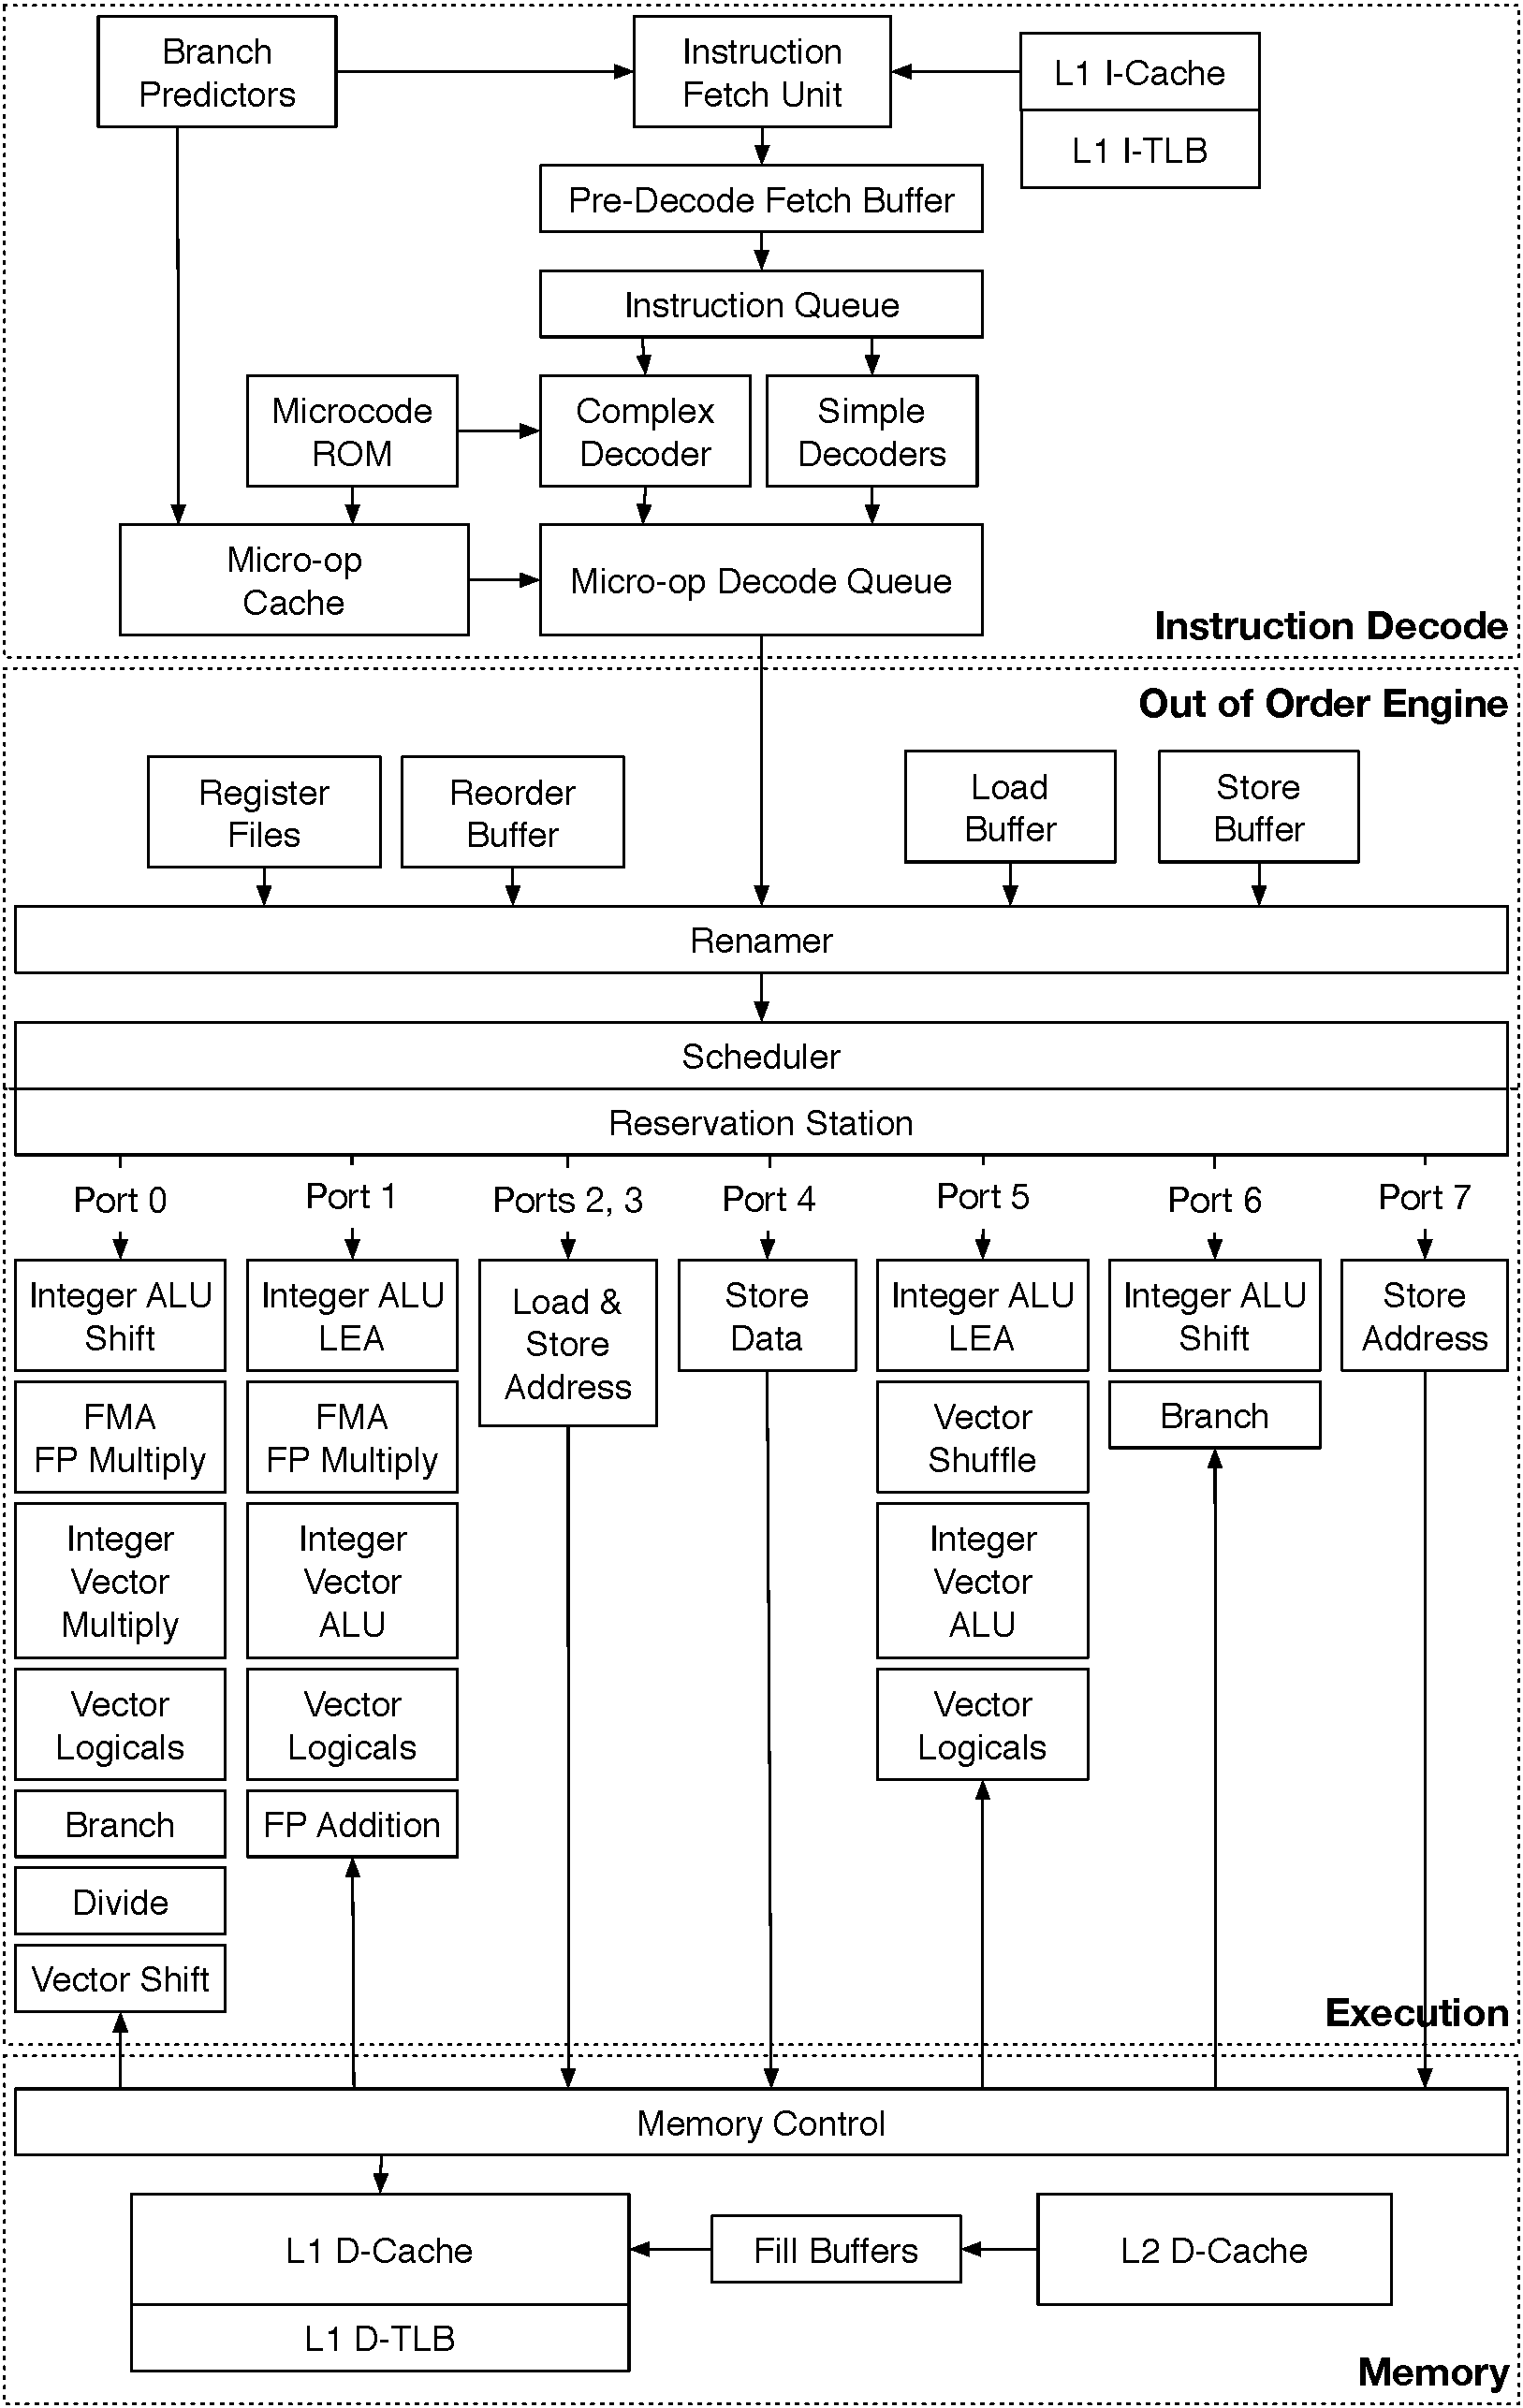
\includegraphics[width=85mm]{figures/cpu_out_of_order.pdf}}
  \caption{
    The structures in a CPU core that are relevant to out-of-order and
    speculative execution. Instructions are decoded into micro-ops, which are
    scheduled on one of the execution unit's ports. The branch predictor
    enables speculative execution when a branch is encountered.
  }
  \label{fig:cpu_out_of_order}
\end{figure}

% Intel Microarchitecture Code Name Sandy Bridge Pipeline Overview:
%     Optimization S 2.2.1
% The Front End: Optimization S 2.2.2

The x86 architecture defines a \textit{complex instruction set} (CISC).
However, virtually all modern CPUs are architected following \textit{reduced
instruction set} (RISC) principles. This is accomplished by having the
instruction decode stage break down each x86 instruction into
\textit{micro-ops}. The other stages of the execution pipeline work exclusively
with micro-ops.

% Out of Order Engine: Optimization S 2.2.23
% Renamer: Optimization S 2.2.3.1
% Scheduler: Optimization S 2.2.3.2



% Modern Intel processors use register renaming to implement out of order
% execution, so the registers making up the execution context do not address
% fixed entries in the register file. Out of order execution, described in
% \cite{patterson2013architecture} and \cite{hennessy2012architecture}, can be
% ignored when understanding SGX. However, its effects must be taken into account
% when conducting timing attacks.


% Branch Prediction: Optimization S 2.2.2.3

% Data Prefetching: Optimization S 2.2.5.4
